\documentclass{article}

\usepackage{graphicx}
\usepackage{tikz}
\usepackage{tikzsymbols}
\usetikzlibrary{calc,patterns,shapes.geometric}
\pagestyle{empty}
\usepackage[margin=0pt]{geometry}
\geometry{papersize={14in,12in}}

\def\centerarc[#1](#2)(#3:#4:#5){\draw[#1] ($(#2)+({#5*cos(#3)},{#5*sin(#3)})$) arc (#3:#4:#5);}

\begin{document}
	\begin{figure}
		\centering
		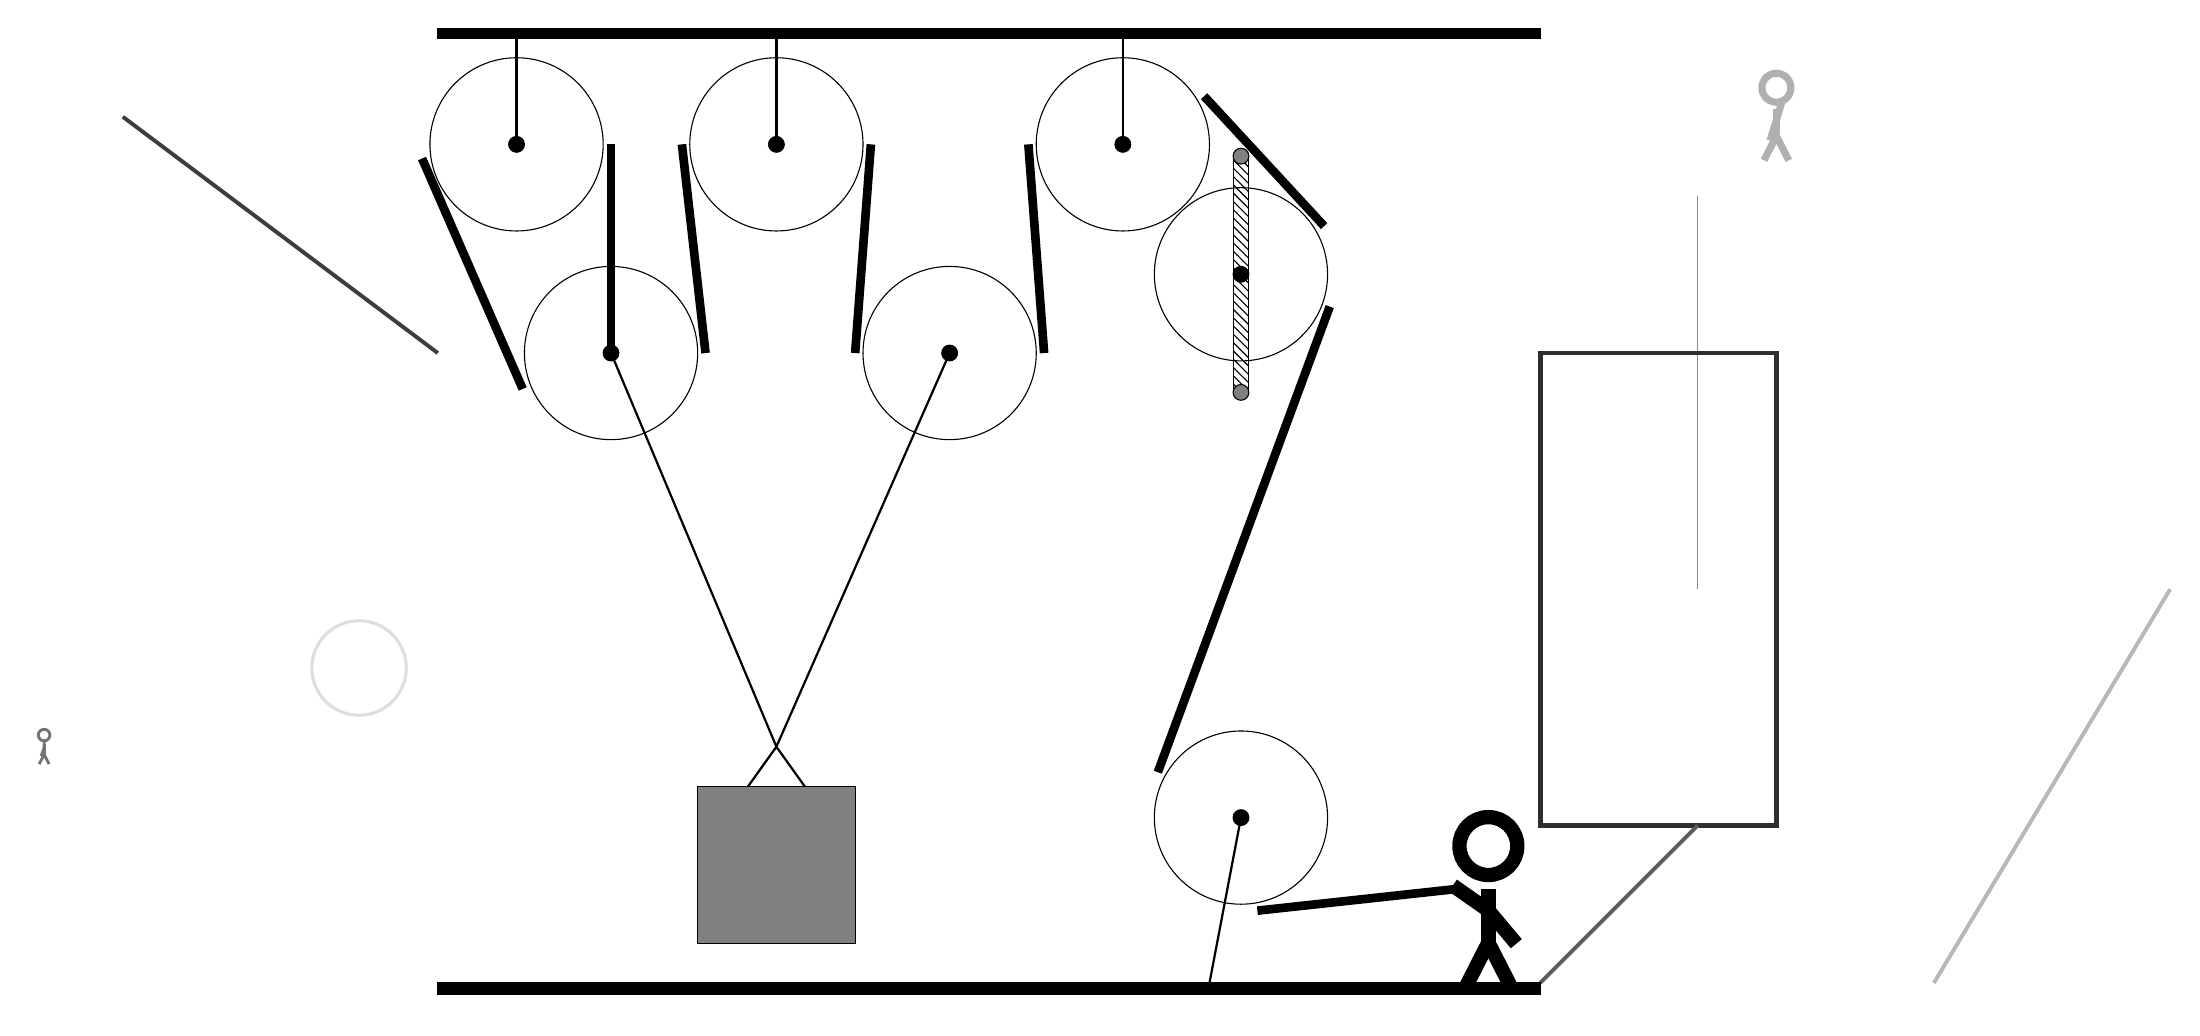
\begin{tikzpicture}
			%%%%% START %%%%%
			
			\draw[fill=black] (-2, 9) rectangle (12, 9.125);
			
			\draw (-1, 7.65) circle (1.1);
			\draw[fill=black] (-1, 7.65) circle (0.1);
			\draw[thick] (-1, 7.65) -- (-1, 9);
			
			\draw (2.3, 7.65) circle (1.1);
			\draw[fill=black] (2.3, 7.65) circle (0.1);
			\draw[thick] (2.3, 7.65) -- (2.3, 9);
			
			\draw [line width=0.4mm, color=black!13](-3, 1) circle (0.6);
			
			\draw[line width=0.5mm, color=black!76](-2, 5) -- (-6, 8);
			\node[line width=0.2mm, color=black!55] at (-7, 0) {\Strichmaxerl[2][70][89]};
			\draw [line width=0.5mm, color=black!24](-6, 4) circle (0.0);
			
			\draw[line width=0.2mm, color=black!46] (14, 7) rectangle (14, 2);
			\draw[line width=0.5mm, color=black!65](12, 0) -- (12, 2);
			\draw[line width=0.5mm, color=black!28](17, -3) -- (20, 2);
			\node[line width=0.6mm, color=black!31] at (15, 8) {\Strichmaxerl[5][73][73]};
			\draw[line width=0.6mm, color=black!82] (12, 5) rectangle (15, -1);
			\draw[line width=0.5mm, color=black!64](14, -1) -- (12, -3);
			
			\draw (6.7, 7.65) circle (1.1);
			\draw[fill=black] (6.7, 7.65) circle (0.1);
			\draw[thick] (6.7, 7.65) -- (6.7, 9);
			
			\draw (0.2, 5) circle (1.1);
			\draw[fill=black] (0.2, 5) circle (0.1);
			
			\draw (4.5, 5) circle (1.1);
			\draw[fill=black] (4.5, 5) circle (0.1);
			
			\draw (8.2, 6) circle (1.1);
			\draw[fill=black] (8.2, 6) circle (0.1);
			\draw[pattern=north west lines, pattern color=black] (8.1, 7.5) rectangle (8.3, 4.5);
			\draw[fill=black!50] (8.2, 7.5) circle (0.1);
			\draw[fill=black!50] (8.2, 4.5) circle (0.1);
			
			\draw (8.2, -0.9) circle (1.1);
			\draw[fill=black] (8.2, -0.9) circle (0.1);
			\draw[thick] (8.2, -0.9) -- (7.8, -3);
			
			\draw[thick] (0.2, 5) -- (2.3, 0)  -- (4.5, 5);
			\draw[thick]  (1.8, -0.7) -- (2.3, 0) -- (2.8, -0.7);
			\draw[fill=black!50] (1.3, -0.5) rectangle (3.3, -2.5);
			\draw[line width=1.1mm] (0.2, 5) -- (0.2, 7.65);
			\centerarc[line width=1.1mm](-1, 7.65)(0:200:1.2000000000000002);
			\draw[line width=1.1mm] (-2.2, 7.47) -- (-0.922, 4.544);
			\centerarc[line width=1.1mm](0.2, 5)(200:360:1.2000000000000002);
			\draw[line width=1.1mm](1.4, 5) -- (1.1, 7.65);
			\centerarc[line width=1.1mm](2.3, 7.65)(0:180:1.2000000000000002);
			\draw[line width=1.1mm] (3.5, 7.65) -- (3.3, 5);
			\centerarc[line width=1.1mm](4.5, 5)(180:360:1.2000000000000002);
			\draw[line width=1.1mm] (5.7, 5) -- (5.5, 7.65);
			\centerarc[line width=1.1mm](6.7, 7.65)(30:180:1.2000000000000002);
			\draw[line width=1.1mm](7.732, 8.262) -- (9.256, 6.612);
			\centerarc[line width=1.1mm](8.2, 6)(160:211:-1.2000000000000002);
			\draw[line width=1.1mm](9.3276, 5.5896) -- (7.144, -0.324);
			\centerarc[line width=1.1mm](8.2, -0.9)(150:280:1.2000000000000002);
			\draw[line width=1.1mm](8.4083, -2.0818) -- (11, -1.8);
			
			\node at (11.3, -2) {\Strichmaxerl[10][-35][-50]};
			
			\draw[fill=black] (-2, -3) rectangle (12, -3.15);
			
			%%%%% END %%%%%
		\end{tikzpicture}
	\end{figure}	
\end{document}